%% ============================================================
%%  Chapter: Testing, Expert Annotation and Community Verification
%% ============================================================
\chapter{Testing, Expert Annotation and Community Verification}
\label{sec:verification}

\section{Overview}

The empirical validity of a sign language system depends not only on computational metrics (gloss WER,
boundary F1, back-translation BLEU) but ultimately on the judgment of trained Deaf signers and
qualified sign language educators.  Isharati therefore embeds a structured human-in-the-loop
verification workflow that operates \emph{in parallel} with the automated pipeline.  All 6,112 signs
currently seeded in the PostgreSQL lexicon database are accessible through the \textbf{Review Studio}
--- a dedicated web interface at the live deployment
(\url{https://huggingface.co/spaces/FatimahEmadEldin/isharati-app}) --- where certified annotators
can inspect, approve, flag, modify, or reject individual sign recordings before they are promoted to
the production lexicon.

\section{The Review Studio Interface}
\label{sec:review_studio}

\begin{figure}[ht]
\centering
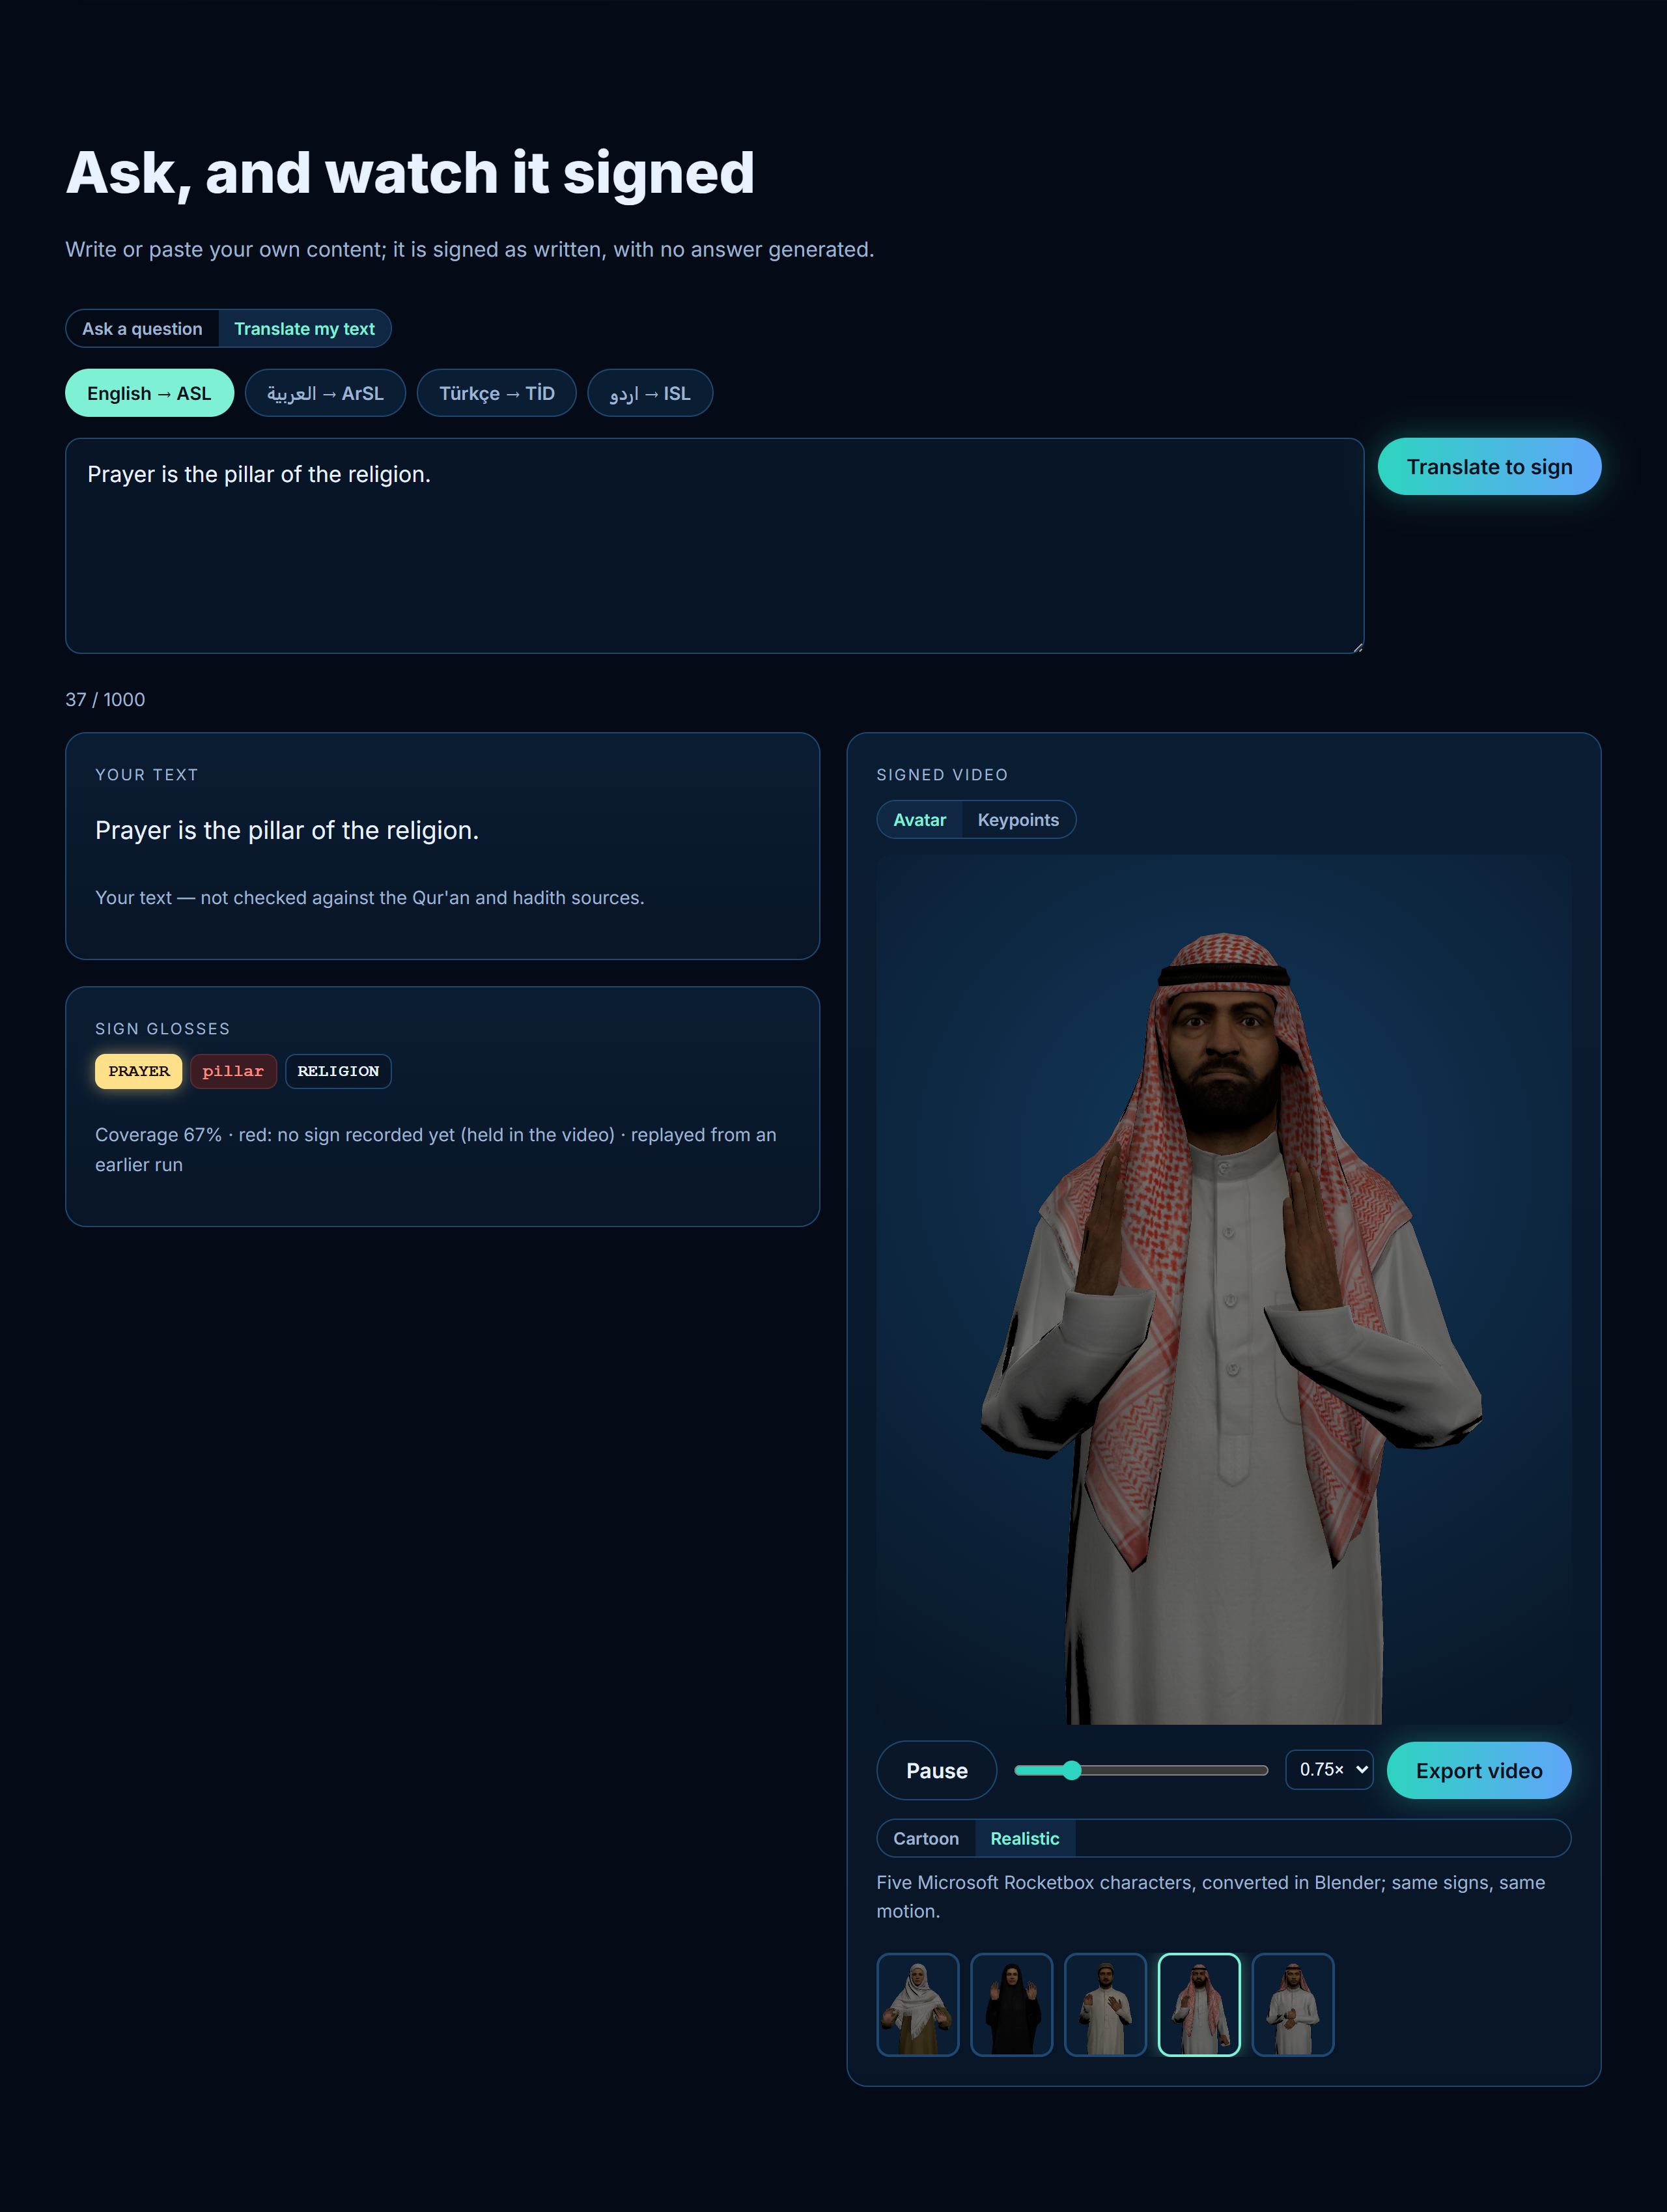
\includegraphics[width=\textwidth]{figures/ui_studio.png}
\caption{\textbf{Isharati Review Studio.}  The dual-panel annotation interface.
\textbf{Left panel:} Review queue of 6,112 seeded signs, filterable by two independent drop-down
menus --- \emph{Review Status} (All Signs, Needs Revision / Pending, Approved, Needs Modification,
Rejected) and \emph{Collection / Dataset} (12 collections listed in Table~\ref{tab:review_collections}).
Each queue entry shows the Arabic gloss, its colour-coded status badge, and the source dataset tag.
\textbf{Right panel:} Sign playback studio --- side-by-side 3D avatar rendering and skeletal keypoint
overlay, transport controls (play/pause, scrub bar, speed selector 0.5$\times$, 0.75$\times$,
1$\times$), and the three annotator decision buttons (Approved, Needs Modification, Rejected) with a
free-text notes field.  An integrated webcam recording module lets an expert re-record a corrected
physical gesture on the spot and upload it to the dataset repository.}
\label{fig:review_studio}
\end{figure}

\subsection{Dual-Axis Filtering}

The queue panel exposes two cascading filters:
\begin{enumerate}[leftmargin=*,itemsep=2pt]
  \item \textbf{Review Status filter} --- selects signs by their current verification state:
    \emph{All Signs} (6,112 total),
    \emph{Needs Revision / Pending},
    \emph{Approved},
    \emph{Needs Modification}, or
    \emph{Rejected}.
  \item \textbf{Collection / Dataset filter} --- restricts the queue to one of the 12 source
    collections (Table~\ref{tab:review_collections}).
\end{enumerate}
Applying both filters simultaneously (e.g., ``Pending signs from the Broadcast Sources collection'')
produces a targeted work-list that lets annotators focus on the highest-priority gaps without
wading through already-approved material.

\begin{table}[ht]
\centering\small
\caption{The 12 sign collections exposed in the Review Studio dataset filter, with their seeded
sign counts and extraction modality.  The \emph{Isharah Corpus Mined} row holds the 1,113
glosses mined from continuous Saudi Sign Language sentences; they were later found to be mis-segmented (Section~\ref{sec:lexicons})
and are excluded from the lexicon until re-mined.}
\label{tab:review_collections}
\begin{tabularx}{\textwidth}{L{4.6cm} r L{2.4cm} Y}
\toprule
Collection & Signs & Modality & Notes \\
\midrule
New Broadcast Sources & 2,409 & Continuous & 249 broadcast videos, 20 religious channels \\
Unified Arabic Dictionary & 1,283 & Isolated & Pan-Arab standardized dictionary \\
Kuwaiti Sign Dictionary & 975 & Isolated & Gulf and Kuwaiti dialect \\
KArSL Saudi Benchmark & 492 & Isolated & 3 native Deaf Saudi signers \\
Qur'an Curriculum (Al-Kharj) & 305 & Continuous & Word-by-word Qur'anic recitation \\
Tawasol Islamic Center & 196 & Continuous & Islamic pillars \& conversational signs \\
Scouts' Sign Dictionary & 139 & Isolated & Arab Scouting vocabulary \\
Levantine / Jordan Shorts & 110 & Continuous & Jordanian and Palestinian dialect \\
Children's Sign Dictionary & 87 & Isolated & Pediatric and educational signs \\
Arabic Dictionary Explained & 43 & Isolated & Morphological explanations \\
Saudi Dictionary Explained & 39 & Isolated & Saudi linguistic glosses \\
Isharah Corpus Mined & 34 & Continuous & RoPE-extracted continuous Saudi signs \\
\midrule
\textbf{Total} & \textbf{6,112} & & \\
\bottomrule
\end{tabularx}
\end{table}

\subsection{Isolated vs.\ Continuous Sign Inventory}

A critical distinction in the review process is the source modality of each sign recording, because
this directly affects the expected visual quality and review criteria applied by annotators:

\begin{itemize}[leftmargin=*,itemsep=2pt]
  \item \textbf{Isolated signs} (3,019 signs, 49.4\% of the seeded pool) originate from dedicated
    dictionary videos where a single word is performed without surrounding context.  Each recording
    is clean, includes the preparation and retraction strokes, and is labelled directly by the
    dictionary publisher.  Review focuses on handshape accuracy and cultural appropriateness.
  \item \textbf{Continuous segmented signs} (3,093 signs, 50.6\%) were algorithmically extracted
    from long-form signing streams (lessons, broadcasts, recitations) using the RoPE Transformer
    boundary model (Section~\ref{sec:rope_segmentation}).  Automatic segmentation of continuous
    signing is not reliable yet (best boundary F1 within $\pm4$ frames: 44.6\% on synthetic streams,
    Table~\ref{tab:segmentation_benchmark}), so these clips may contain partial strokes, truncated
    holds, or co-articulation bleed from adjacent glosses.  Review of this subset therefore also evaluates segmentation precision
    and temporal completeness.
\end{itemize}

Table~\ref{tab:isolated_vs_continuous} summarises the isolated vs.\ continuous breakdown per
source language and collection:

\begin{table}[ht]
\centering\small
\caption{Isolated vs.\ continuous sign breakdown across the full 6,112-sign review pool.
``Isolated'' denotes dictionary-style single-word recordings; ``Continuous'' denotes signs
extracted by the RoPE Transformer segmentation pipeline from broadcast, recitation, or lesson
streams.}
\label{tab:isolated_vs_continuous}
\begin{tabular}{l r r r}
\toprule
Source Group & Isolated & Continuous & Total \\
\midrule
Islamic Broadcast Sources (20 channels) & 0 & 2,409 & 2,409 \\
Unified Arabic Dictionary & 1,283 & 0 & 1,283 \\
Kuwaiti Sign Dictionary & 975 & 0 & 975 \\
KArSL Saudi Benchmark & 492 & 0 & 492 \\
Qur'an Curriculum (Al-Kharj) & 0 & 305 & 305 \\
Tawasol Islamic Center & 0 & 196 & 196 \\
Scouts' Sign Dictionary & 139 & 0 & 139 \\
Levantine / Jordan Shorts & 0 & 110 & 110 \\
Children's Sign Dictionary & 87 & 0 & 87 \\
Arabic Dictionary Explained & 43 & 0 & 43 \\
Saudi Dictionary Explained & 39 & 0 & 39 \\
Isharah Corpus Mined & 0 & 34 & 34 \\
\midrule
\textbf{Total} & \textbf{3,019} & \textbf{3,093} & \textbf{6,112} \\
\textbf{Share} & \textbf{49.4\%} & \textbf{50.6\%} & \textbf{100\%} \\
\bottomrule
\end{tabular}
\end{table}

\subsection{Playback and Decision Workflow}

Selecting any sign from the queue loads its $[T, 50, 3]$ pose tensor in real time.  The playback
panel renders the sign simultaneously as:
\begin{itemize}[leftmargin=*,itemsep=2pt]
  \item a \textbf{3D VRM avatar} (choice of Rocketbox Male/Female, hijab, shemagh, or thobe
    outfit), with kinematic retargeting applied to the 50 normalized joints;
  \item a \textbf{skeletal keypoint overlay} --- upper-body bones in teal, right-hand 21-joint
    chains in crimson, left-hand chains in sky blue --- using the normalized coordinate frame
    (neck at origin, shoulder-width unit scale).
\end{itemize}
Transport controls support variable playback speeds (0.5$\times$, 0.75$\times$, 1$\times$) and
frame-level scrubbing, enabling precise inspection of hold segments, transition smoothness, and
finger configurations.

Upon review the annotator issues one of three verdicts via the decision buttons:
\begin{enumerate}[leftmargin=*,itemsep=2pt]
  \item \textbf{Approved} --- the sign is accepted as a canonical lexicon entry and promoted to the
    production dataset (\url{https://huggingface.co/datasets/FatimahEmadEldin/isharati-review-signs}).
  \item \textbf{Needs Modification} --- the sign is linguistically valid but requires a technical
    correction (re-trimming, speed normalisation, or coordinate adjustment); the sign is queued
    for automated re-processing.
  \item \textbf{Rejected} --- the sign is incorrect (wrong handshape, wrong gloss label, or
    culturally inappropriate), and is removed from the production candidate pool.
\end{enumerate}
All decisions are written to the Neon PostgreSQL database with a timestamp and reviewer identifier,
providing a full audit trail.

\section{Normalization in the Review Process}
\label{sec:verification_normalization}

Signs displayed in the Review Studio are always shown in their \emph{normalized} form, not as raw
pixel coordinates.  The normalization pipeline (Section~\ref{sec:preproc}) applied before display
includes:
\begin{enumerate}[leftmargin=*,itemsep=2pt]
  \item \textbf{Shoulder-width normalization} --- all signers' bodies are rescaled so the neck
    is the spatial origin and the shoulder width equals one unit, eliminating camera distance and
    body proportion differences between dictionary and broadcast sources.
  \item \textbf{Coordinate system flip} --- the raw screen-space $+Y$-down axis is inverted to
    the anatomically natural $+Y$-up convention used by the 3D avatar skeleton.
  \item \textbf{Palm orientation and quaternion hemisphere continuity} --- an orthonormal palm
    frame $(\mathbf{u}_{\text{palm}}, \mathbf{v}_{\text{palm}}, \mathbf{n}_{\text{palm}})$ is
    constructed per frame; quaternion hemisphere flips that cause ``arm glitching'' during rapid
    wrist rotations are corrected by enforcing $\langle q_t, q_{t-1}\rangle \ge 0$, and angular
    jump spikes exceeding $2.0\,\text{rad}$ are replaced by SLERP interpolation.
  \item \textbf{Torso clearance clamping} --- a dynamic forward clearance boundary prevents hands
    from passing through the avatar's torso or robes ($Z_{\text{wrist}} \ge Z_{\text{shoulder}} +
    0.38 \times L_{\text{arm}}$), eliminating the clipping artifacts that would otherwise appear
    when a compressed skeletal window is rendered at normal avatar proportions.
\end{enumerate}
This means that annotators always see a clean, anatomically stable rendering regardless of the
original recording quality, and their judgment can focus on \emph{linguistic correctness} rather
than technical video artifacts.

\section{Expert Sign Language Annotation}
\label{sec:annotators}

\paragraph{Annotator.} The first expert review was carried out by \textbf{Ahmed Tahir}, a sign language expert
(B.Sc.\ in Computer Science, Arab Open University, Saudi branch) who has worked with the National Center for
Artificial Intelligence (NCAI) on a collaboration project on Saudi Sign Language. He reviewed signs in the Review Studio of the
deployed Space during a recorded online session on 4 October 2026 (Figures~\ref{fig:expert_meeting}, \ref{fig:expert_studio}
and~\ref{fig:expert_signing}), demonstrating the correct form of each sign on camera while judging the avatar's rendering.
Further annotators are being recruited, so that each sign can be judged by more than one expert and agreement measured.

\paragraph{What was reviewed.} The session covered the Qur'an-curriculum source (signs cut from the Al-Kharj Qur'an
curriculum videos, Section~\ref{sec:lexicons}), which supplies many of the Qur'anic content words. Each verdict is written to the
\code{sign\_reviews} table of the Neon PostgreSQL database with the sign identifier, gloss, source, decision and a
timestamp. Table~\ref{tab:expert_verdicts} lists all 22 human verdicts. Of the 3,209 seeded entries, the database also
holds about 2,900 rows marked approved or reviewed automatically when sources were imported (KArSL, new Arabic sources,
numbers and model signs); these are \emph{not} expert judgements and are excluded here. One test entry made while the
tool was being built is excluded too.

\begin{table}[ht]
\centering\small
\caption{Expert verdicts from the first review session (4 October 2026, Qur'an-curriculum signs; source: \code{sign\_reviews}).}
\label{tab:expert_verdicts}
\begin{tabularx}{\textwidth}{L{2.6cm} r Y}
\toprule
Verdict & Signs & Glosses \\
\midrule
Approved & 16 & \ar{الله، أشقى، تقوى، سوى، غشي، نهار، ضحى، مؤصدة، عقبة، غير، صراط، ليلة، صالحة، وجد، أعطى، ليل} \\
Needs modification & 1 & \ar{مسكين} \\
Rejected & 5 & \ar{ذكر، تلى، اسم، عابد، أرض} \\
\midrule
Total & 22 & approval rate 72.7\,\% (16/22); acceptable after correction 77.3\,\% (17/22) \\
\bottomrule
\end{tabularx}
\end{table}

\paragraph{What the verdicts changed.} The rejections were acted on straight away:
\begin{itemize}[leftmargin=*,itemsep=2pt]
  \item \ar{عابد} (worshipper) was rejected as a sign. On the expert's advice it is now \emph{fingerspelled}
    letter by letter (\ar{ع ا ب د}) from the KArSL letter signs, recorded as a reviewed decision
    (\code{reviewed\_fingerspelling}), and the same treatment was extended to 22 names of the Companions
    (Section~\ref{sec:ar_norm}).
  \item \ar{ذكر}: the rejected clip turned out to be shared between two senses of the word (\emph{remembrance} and
    \emph{male}); the SignBank rows that reused it for \ar{الرجل} were later rejected for the same reason
    (Section~\ref{sec:ar_norm}).
  \item The remaining rejected signs stay out of production until they are re-recorded or replaced from another source.
\end{itemize}

\begin{figure}[ht]
\centering
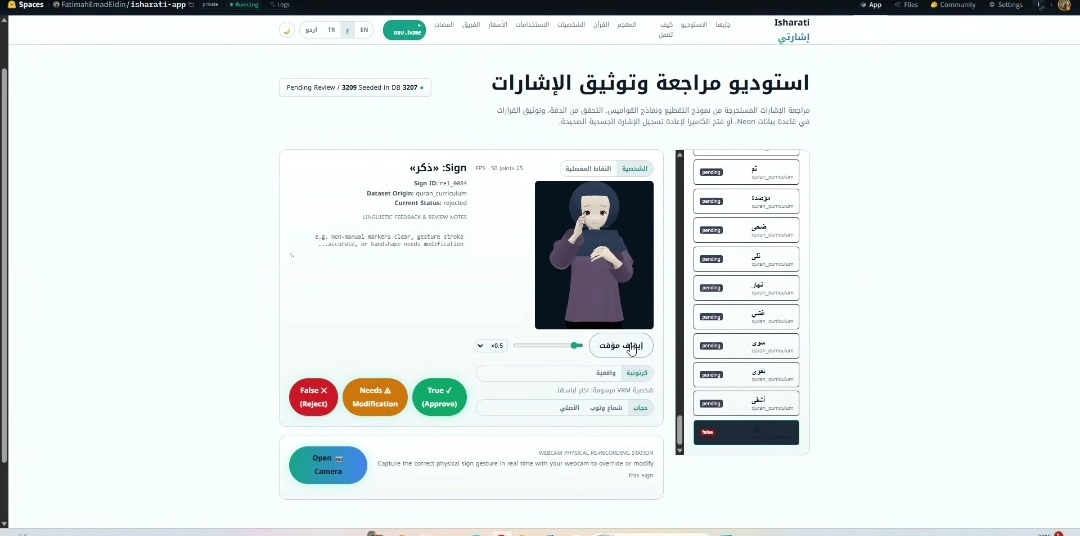
\includegraphics[width=0.49\textwidth]{figures/expert_review/studio_dhikr_rejected.jpg}\hfill
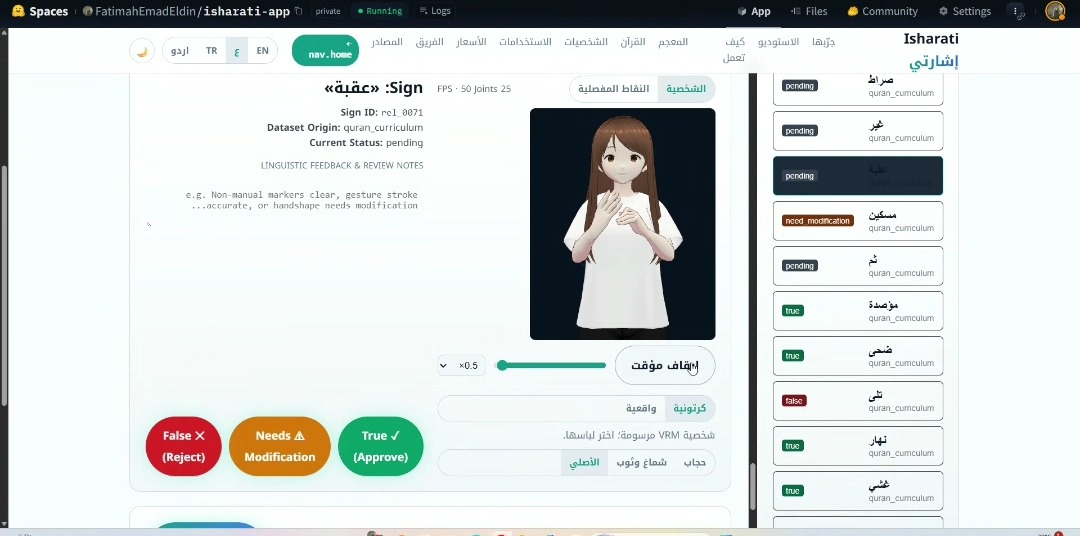
\includegraphics[width=0.49\textwidth]{figures/expert_review/studio_aqaba.jpg}
\caption{The Review Studio during the expert session. Left: \ar{ذكر}, rejected. Right: \ar{عقبة} played on the
cartoon avatar at 0.5$\times$, with the verdict buttons (False / Needs modification / True) and the queue of
Qur'an-curriculum signs with their statuses.}
\label{fig:expert_studio}
\end{figure}

\begin{figure}[ht]
\centering
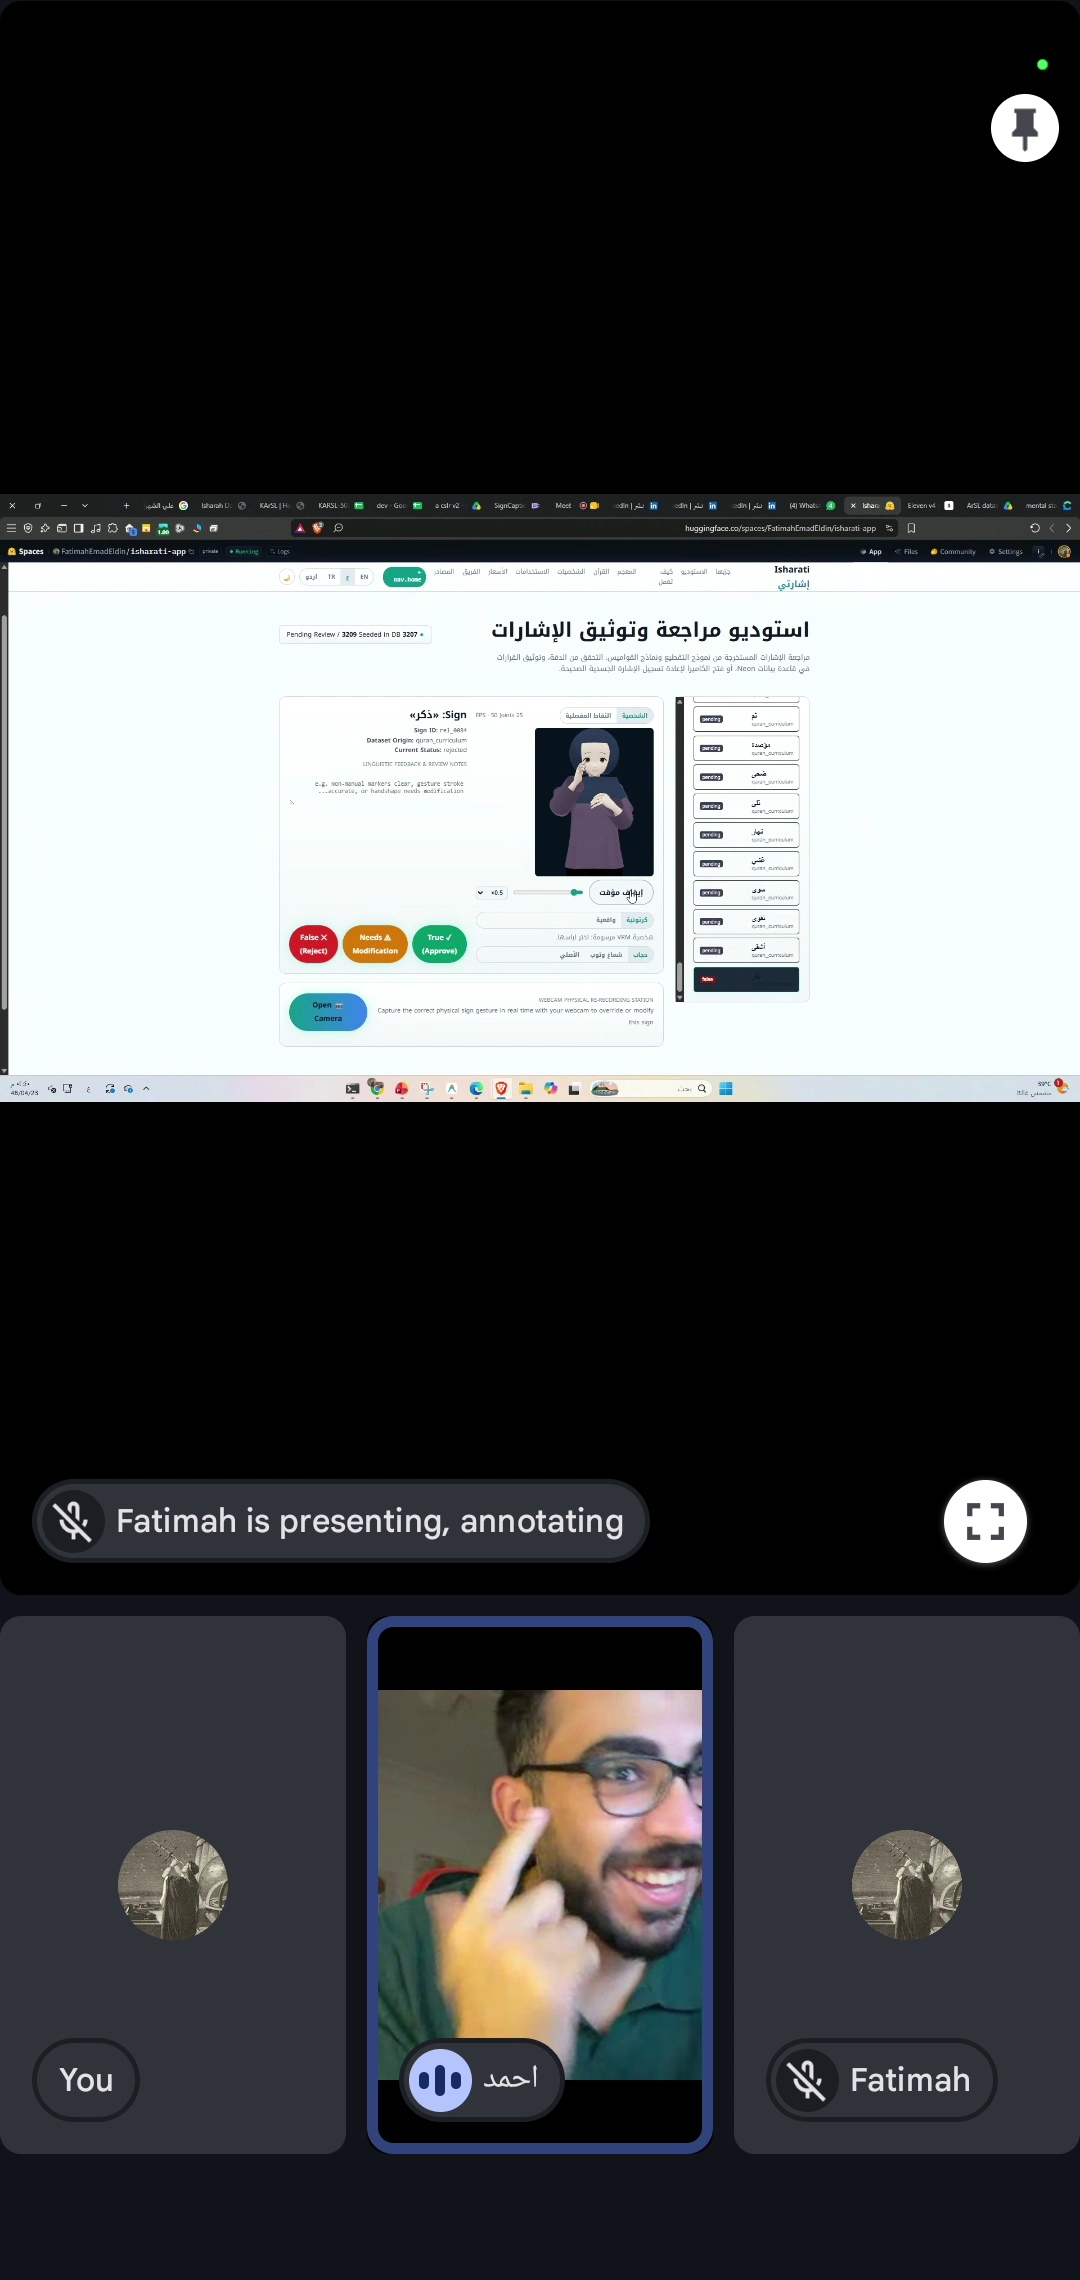
\includegraphics[width=0.32\textwidth]{figures/expert_review/meeting_full_1.jpg}\hfill
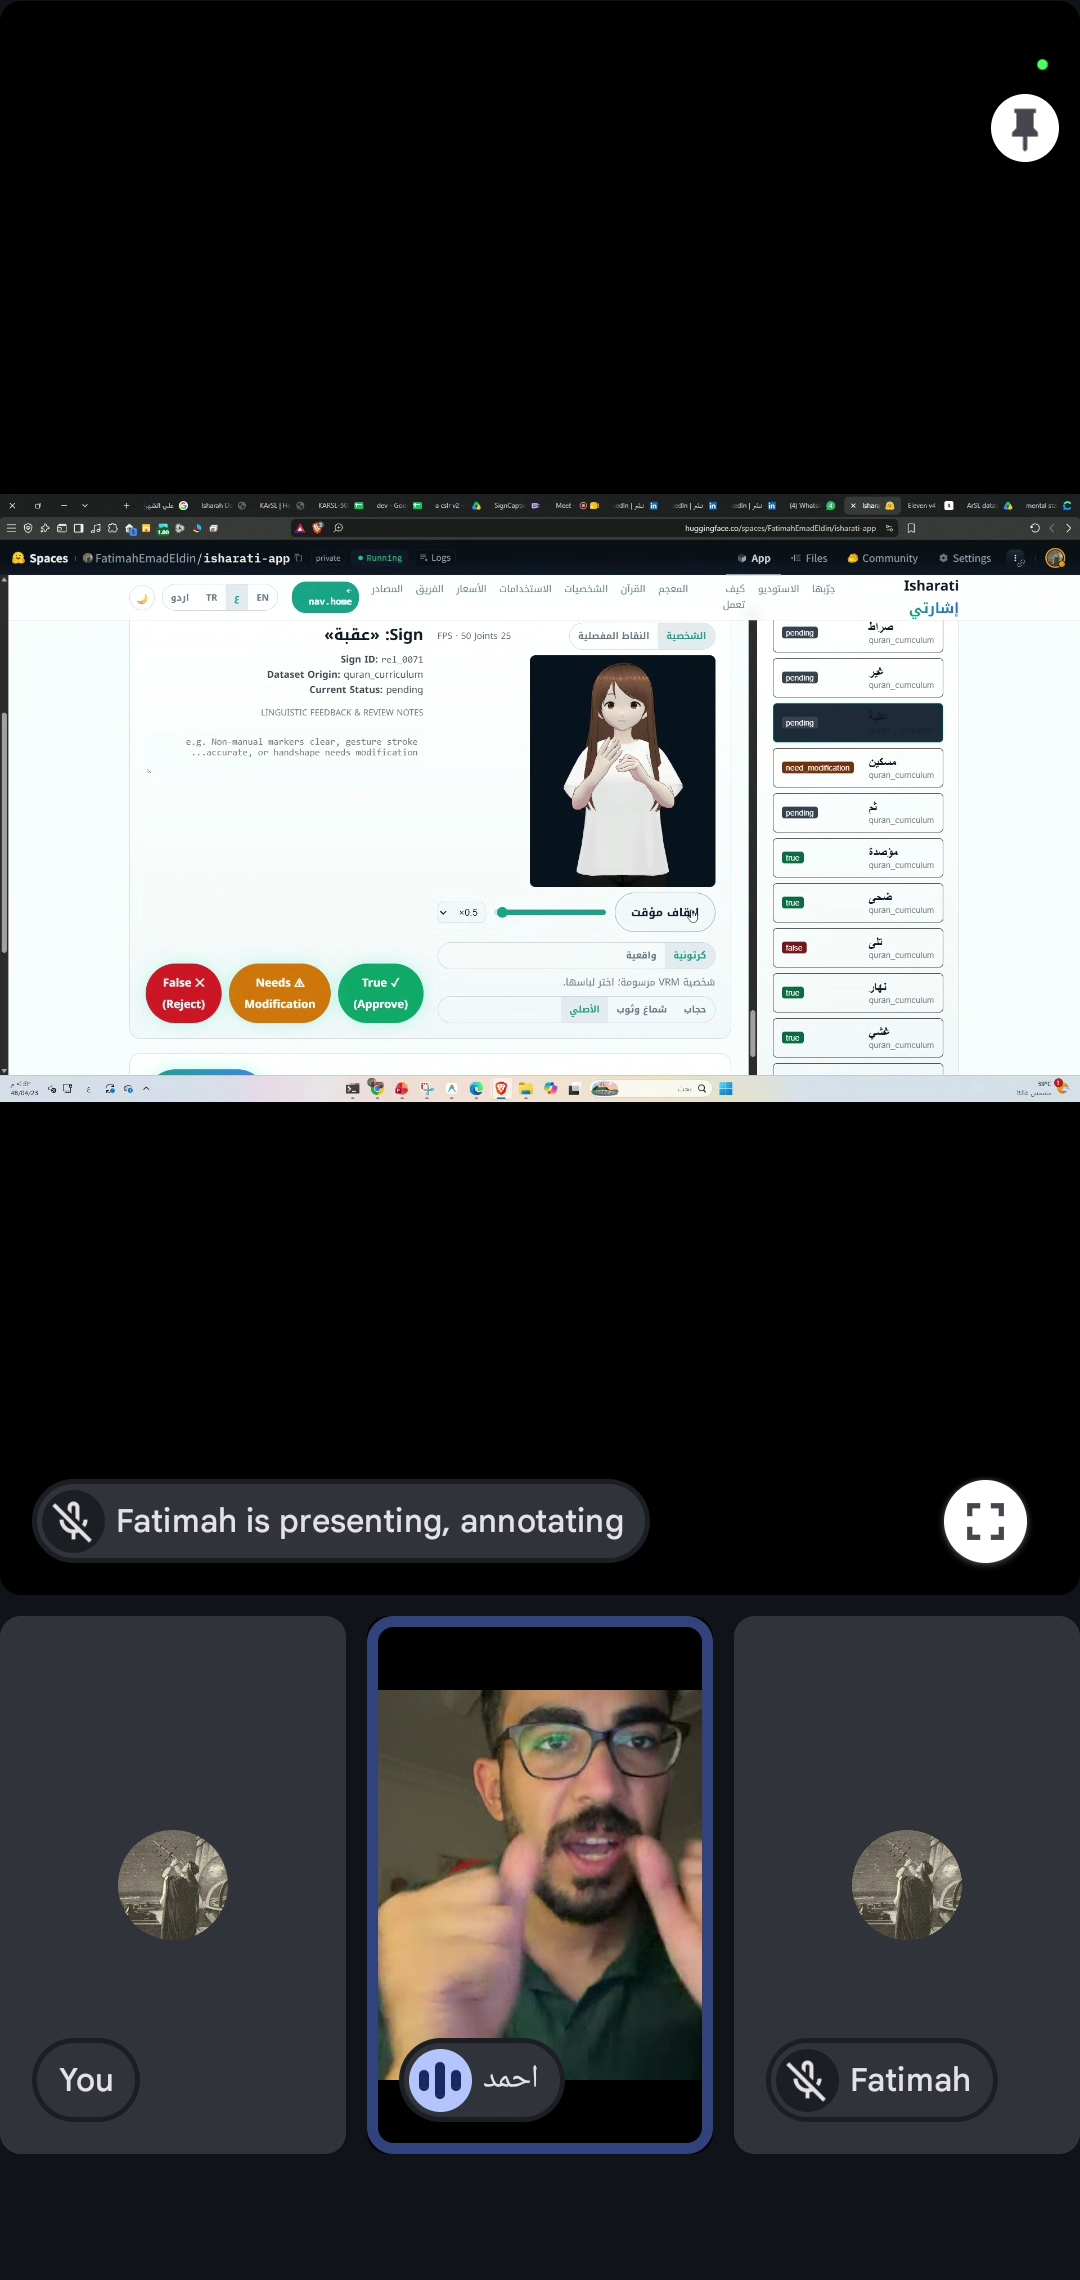
\includegraphics[width=0.32\textwidth]{figures/expert_review/meeting_full_2.jpg}\hfill
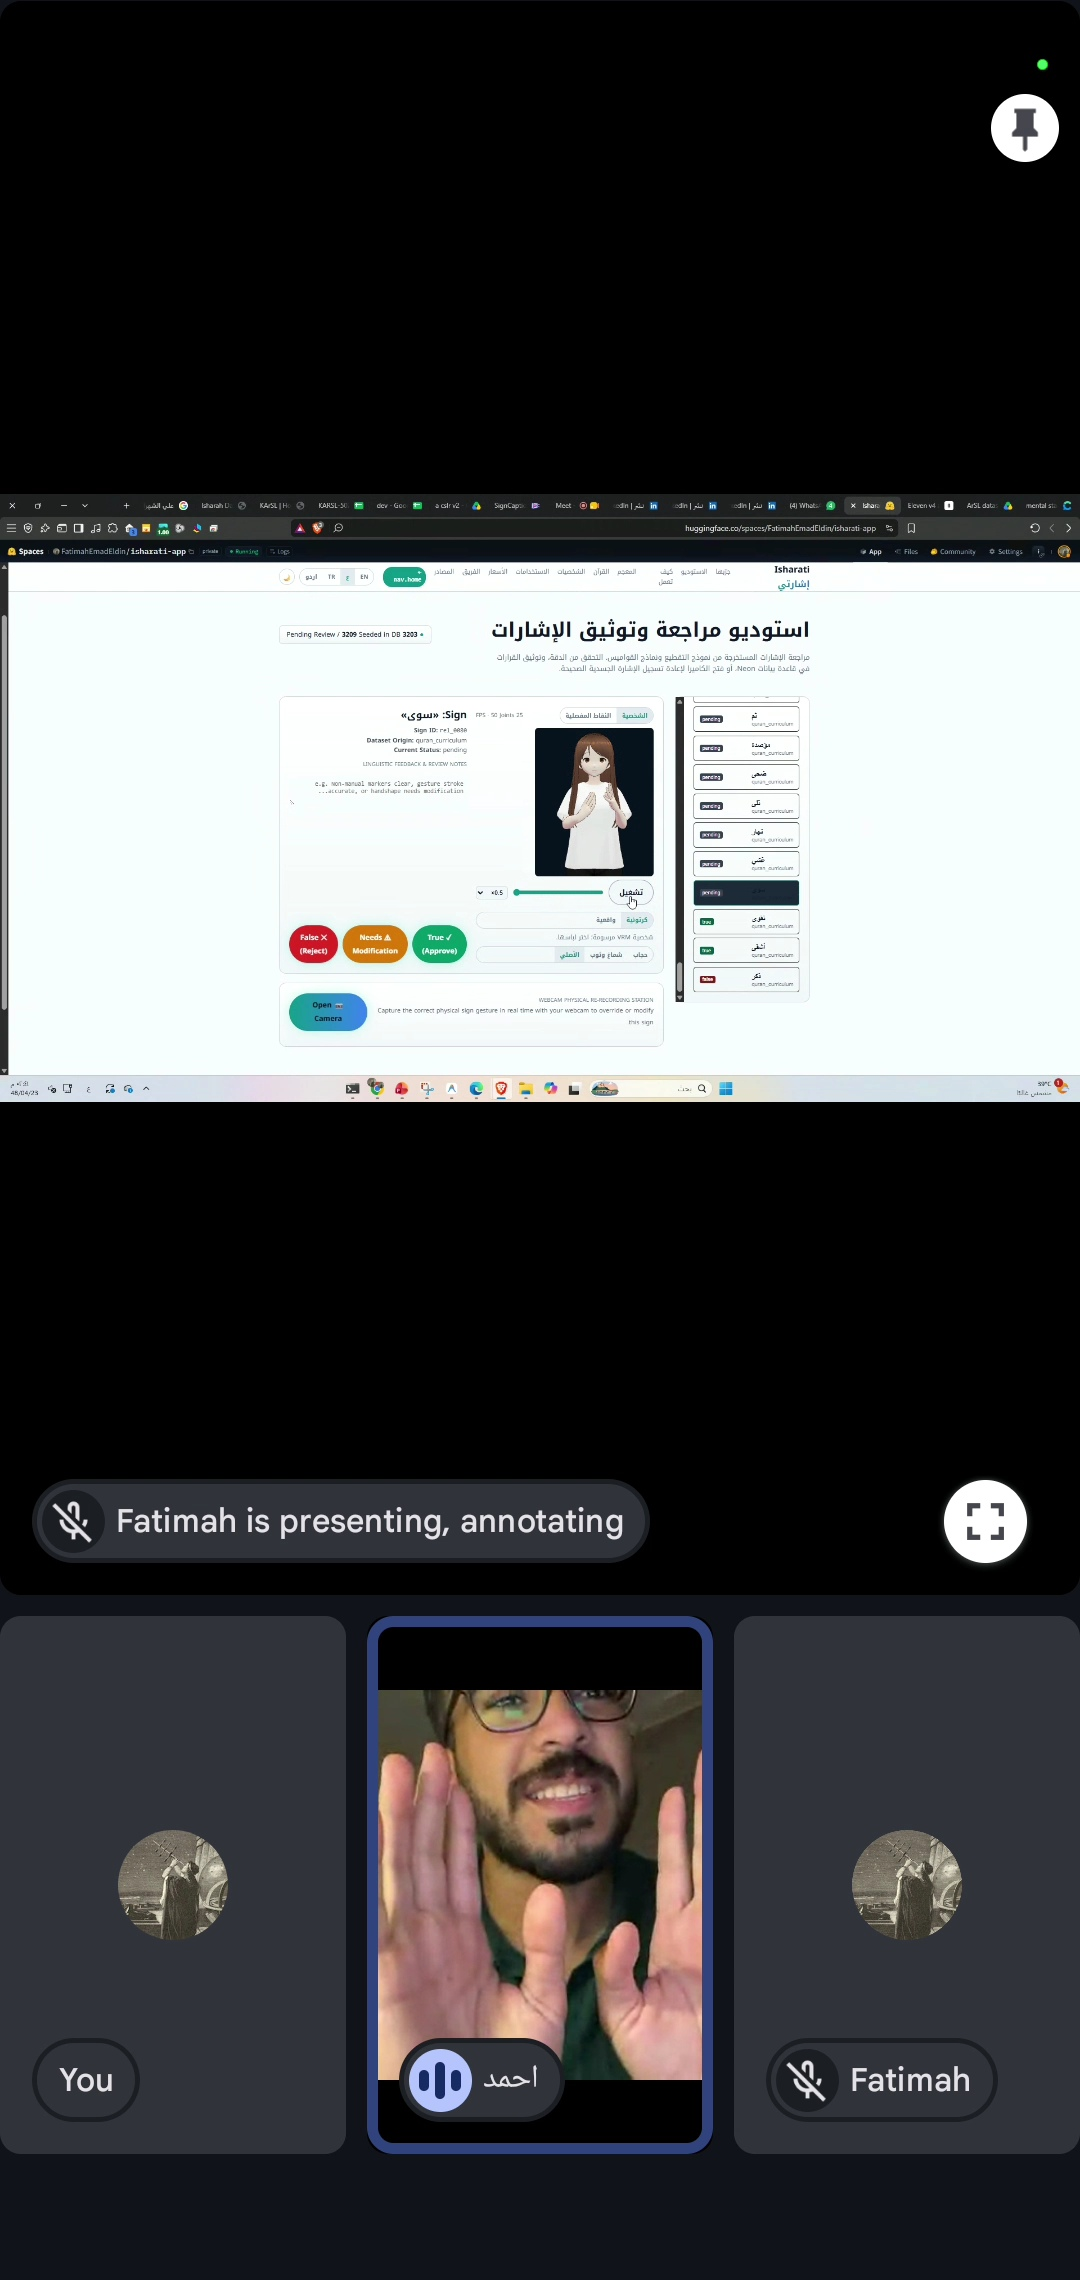
\includegraphics[width=0.32\textwidth]{figures/expert_review/meeting_full_3.jpg}
\caption{The online review session of 4 October 2026, uncropped: the Review Studio shared on screen while the expert, Ahmed
Tahir, demonstrates each sign on camera.}
\label{fig:expert_meeting}
\end{figure}

\begin{figure}[ht]
\centering
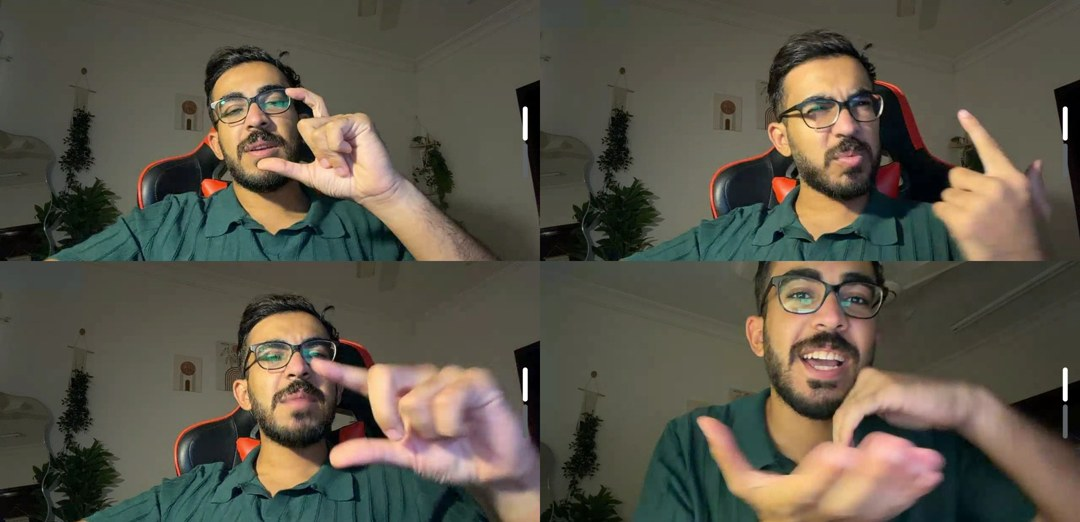
\includegraphics[width=0.8\textwidth]{figures/expert_review/expert_signing_grid.jpg}
\caption{The expert demonstrating signs on camera during the review session, used to judge and correct the avatar's
handshapes.}
\label{fig:expert_signing}
\end{figure}

\paragraph{Limits.} This is one expert and 22 signs: enough to catch systematic problems (the shared-clip sense error,
the need to fingerspell a word), not to estimate the precision of the whole lexicon. The next step is a stratified
sample across sources, judged by at least two experts, with inter-annotator agreement reported.

\section{Summary}

The Review Studio turns the automatically built lexicon into one that experts can check sign by sign, with every
decision stored and traceable. The first expert session approved 16 of 22 signs, and its rejections led directly to
fixes in the lexicon (fingerspelling and the removal of a shared clip with two meanings). The review is ongoing; verified signs will be released
in the \code{isharati-review-signs} Hugging Face dataset with the annotation log (reviewer, timestamp, decision, notes).
